%!TEX root = ../../main.tex
\section{1D scatter curve similarity analysis}
\label{sec:1D scatter curve similarity analysis}
To increase the signal to noise ratio when processing data in SAXS it is necessary to merge 1D intensity curves from several frames.
If the scattering for different frames is coming from the same molecule in sample then the frames will be similar i.e. the frames will overlap.
However as radiation damage progresses during the experiment, the protein begin to aggregate.
This aggregation causes the intensity curve to change (), therefore it is necessary to determine the similarity between any two pairs of frames to determine which frames to merge.
\begin{figure}
    \centering
    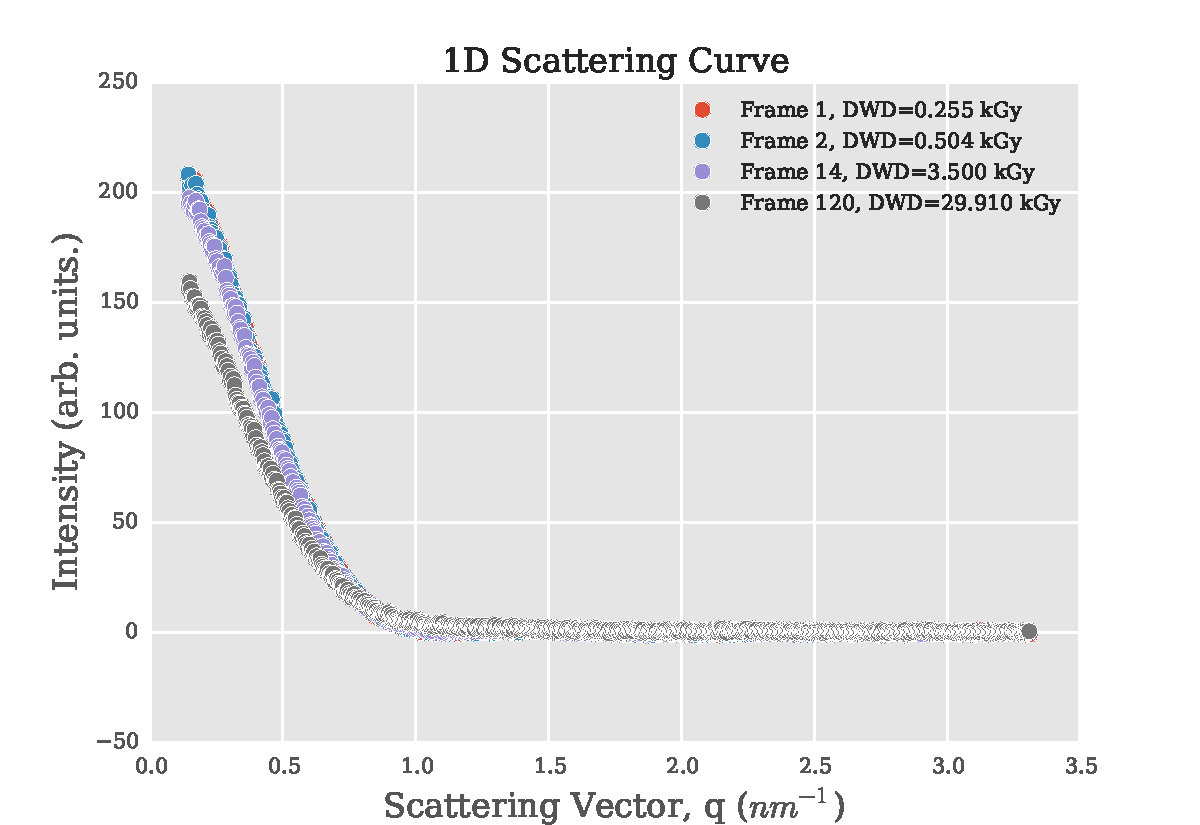
\includegraphics[width=0.8\textwidth]{figures/saxs/scatter_curves.pdf}
    \caption{1D scattering curves from the first run of the GI sample with no radioprotectant compounds added. Frames 1 and 2 are considered similar so these curves clearly overlap. Frame 14 is the first frame considered dissimilar to the first frame. By visual inspection the dissimilarity is not obvious. Frame 120 was the last frame collected in this run and it is clear that the molecules in the sample have undergone significant structural changes due to the obvious dissimilarity of frame 120 with the other frames.}
    \label{fig:1D Scatter Curves}
\end{figure}

\subsection{Old method}
\label{sub:Old method}
DATCMP is a software program, distributed as part of the ATSAS suite of software programs for SAXS data processing \cite{petoukhov2012new}, that assesses the similarity between SAXS frames.
The reduced $\chi^2$ statistic \cite{pearson1900x} was the standard method to do this and is given by:
\begin{equation}
    \chi^2 = \f{1}{n-1} \sum_{k=1}^{n}\left[ \f{I_i(q_k) - I_j(q_k)}{\sigma(q_k)}\right]^2
\end{equation}
where $n$ is the number of data points $k$, $I_i(q_k)$ and $I_j(q_k)$ are the intensities at the scattering vector direction $q_k$ for two different frames $i$ and $j$ (the scattering vector is defined in equation \ref{eq:momentum transfer}), and $\sigma(q_k)$ is the error at the $k^{th}$ data point \cite{franke2015synchrotron}.
$\chi^2 = 0$ implies that two scattering profiles are identical, $0.9 \le \chi^2 \le 1.1$ still suggests good agreement between two frames.
$\chi^2 >> 1$ suggests that two frames are very dissimilar.
The frame with the lowest dose is the first frame so it is assumed that the first frame is of the best quality.
Therefore all subsequent frames are compared to the first frame and any frames that show dissimilarity to the first are discarded for further data processing.

This analysis was applied to SAXS data that was collected
